\documentclass[a4paper]{article}

\usepackage[english]{babel}
\usepackage[utf8]{inputenc}
\usepackage{amsmath}
\usepackage{graphicx}
\usepackage[colorinlistoftodos]{todonotes}

\title{CS686 Data Visualization Final Project Report}

\author{Seimei Matsusaki \\ Pan Wang}

\date{\today}

\begin{document}
\maketitle

\begin{abstract}
We visualized “Shelter" database given by our community partner, One World. Our approach is to merge different data visualizations into a single unit. We experienced failures, but our final visualization finally becomes a powerful and convinced proof of One World’s contributions to the improvement of children’s shelter conditions. Although it is not clear how real audience (potential donors) react to our visualization, we believe that it will help One World to attract more external donors.

\end{abstract}

\section{Introduction}
\subsection{Goal}
From our perspective, the goal is to create a visualization to show how much our community partner has contributed to the improvement of shelter conditions for children around the world. From our client's perspective, the goal is to attract more external donors, using our visualization.
\subsection{What we tried to do}
For the alpha release, we created visulizations (e.g., barcharts, geomap) in Tableau, and were going to merge them into one later. However, we found that it was not exactly what the community partner expected us to make; what it really needed was a web-based and interactive visualization, not static one. Therefore, we entirely recreated our visulization in D3. As a result, our early visualizations are no longer used, yet their idea (i.e., integration of different visualizations) is reflected in the new visualization.


\section{Approach}
\label{sec:examples}
\subsection{What approach(es) we used}
As briefly described above, we tried to combine geomap with other charts. This means that we use the map as the user-interface, and other charts (i.e., barchart and stacked bar chart) are shown as a result of the user interaction. Simply put, when user clicks a country, the map will zoom-in and show the corresponding data to the country.
\subsection{Under what circumstances we think it should work well}
Basically there are two circumstances that we think that our visualization work well: when enough data is available to show in the geopmap, and when our visualization is planned to be updated.
\subsection{Why we think it should work well under those circumstances}
Firstly, if enough data is given, the geo-visualiztion can become better than other visualizations: The user easily can understand with which country our community partner works and see its influence around the globe at a glace. Secondly, if the visualization will be updated, data charts can be a matter. In the future, our community partner may want to show a different type of charts instead of the current charts. In such a case, since our geomap UI is independent from chart types, it is easy to connect a new chart with the UI instead. Besides, even though the number of countries increases, it is not required to make a new navigation interface. In the geomap UI, what is necessary then is just to color new countries and connect them to the corresponding data.

\section{Methodology}
\subsection{Map(to show partners in different countries)}
\begin{itemize}
\item What we implemented:
Tooltip to show an overview of the country data; Zoom-In and Zoom-Out functionality.\\
\item What we did not implement: 
In early stages, we planned to place barcharts inside the boundary of a country, not the right side. Yet we realized that some countries such as East Timor were too small to put charts inside.\\
\item Possible alternatives:
It is possible to use a list as an alternative. It is easy to implement since it only requires text. Still, it may need a page navigator when the amount of data increases. As a result, the user may need additional steps to see details. That can lead a bad user experience.
\end{itemize}

\subsection{Bar charts}
\begin{itemize}
\item What we implemented: 
Vertical barcharts.\\
\item What we did not implement: 
Horizontal Bar Charts in order to show the geomap(UI) bigger for better user experience\\
\item Possible alternatives: 
if values had been ordered by the time, we would have used another chart such as line chart. Yet, the actual values are not ordered by specific values, so we wonder if there are barchart alternatives here.
\end{itemize}

\subsection{Stacked Bar Charts}
\begin{itemize}
\item What we implemented: Vertical stacked barcharts.\\
\item What we did not implemente: Horizontal stacked barcharts for the same reason as the barchart.\\
\item Possible alternatives: Grouped bar charts or multiple bar charts could be used for this part. As compared to the stacked barchart, their values are easy to be compared. Still, it becomes difficult to fit in a limited space instead. Since we wanted to show the UI bigger, this aspect was not ignorable. Therefore, we chose the stacked barchart.
\end{itemize}

\section{Demo and Results}
\subsection{demo}
Figure 1 shows the first screen tha the user will see. Only countries that have the corresponding data are colored. The stacked bar chart at the right side shows world data, rather than data associated with specific countries. There are three buttons on the upper right corner. These allow the use to click and switch different datasets: Shelter, Education and Healthcare. The user also can click any contries they want to see. If the corresponding data is available, it is shown as a barchart at the right side (See, Figure 2). If it is not, "NO DATA" notice is shown instead. In either case, when a country is clicked, the map zooms in. If clicked one more time, the map zooms out.

\begin{figure}
\centering
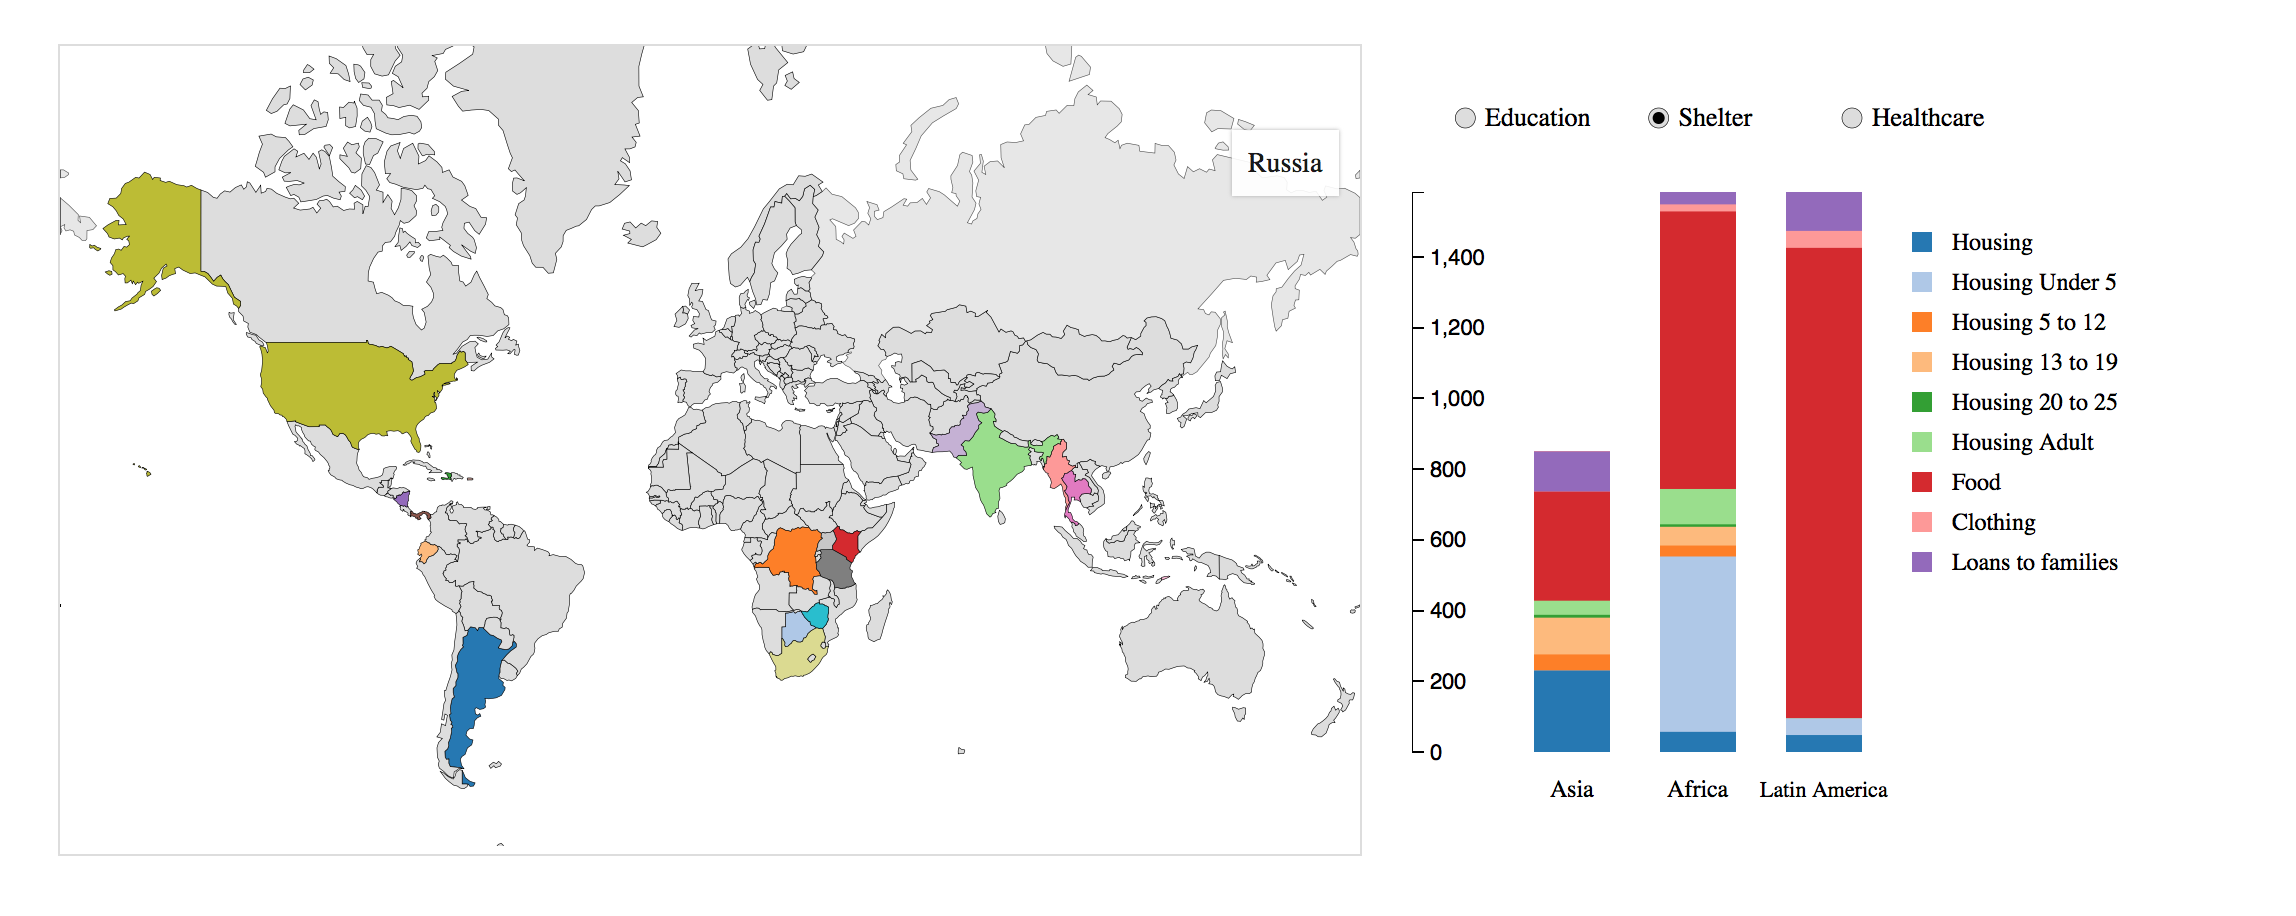
\includegraphics[width=0.7\textwidth]{4.png}
\caption{\label{fig:4} Geomap and Stacked Bar chart}
\end{figure}

\begin{figure}
\centering
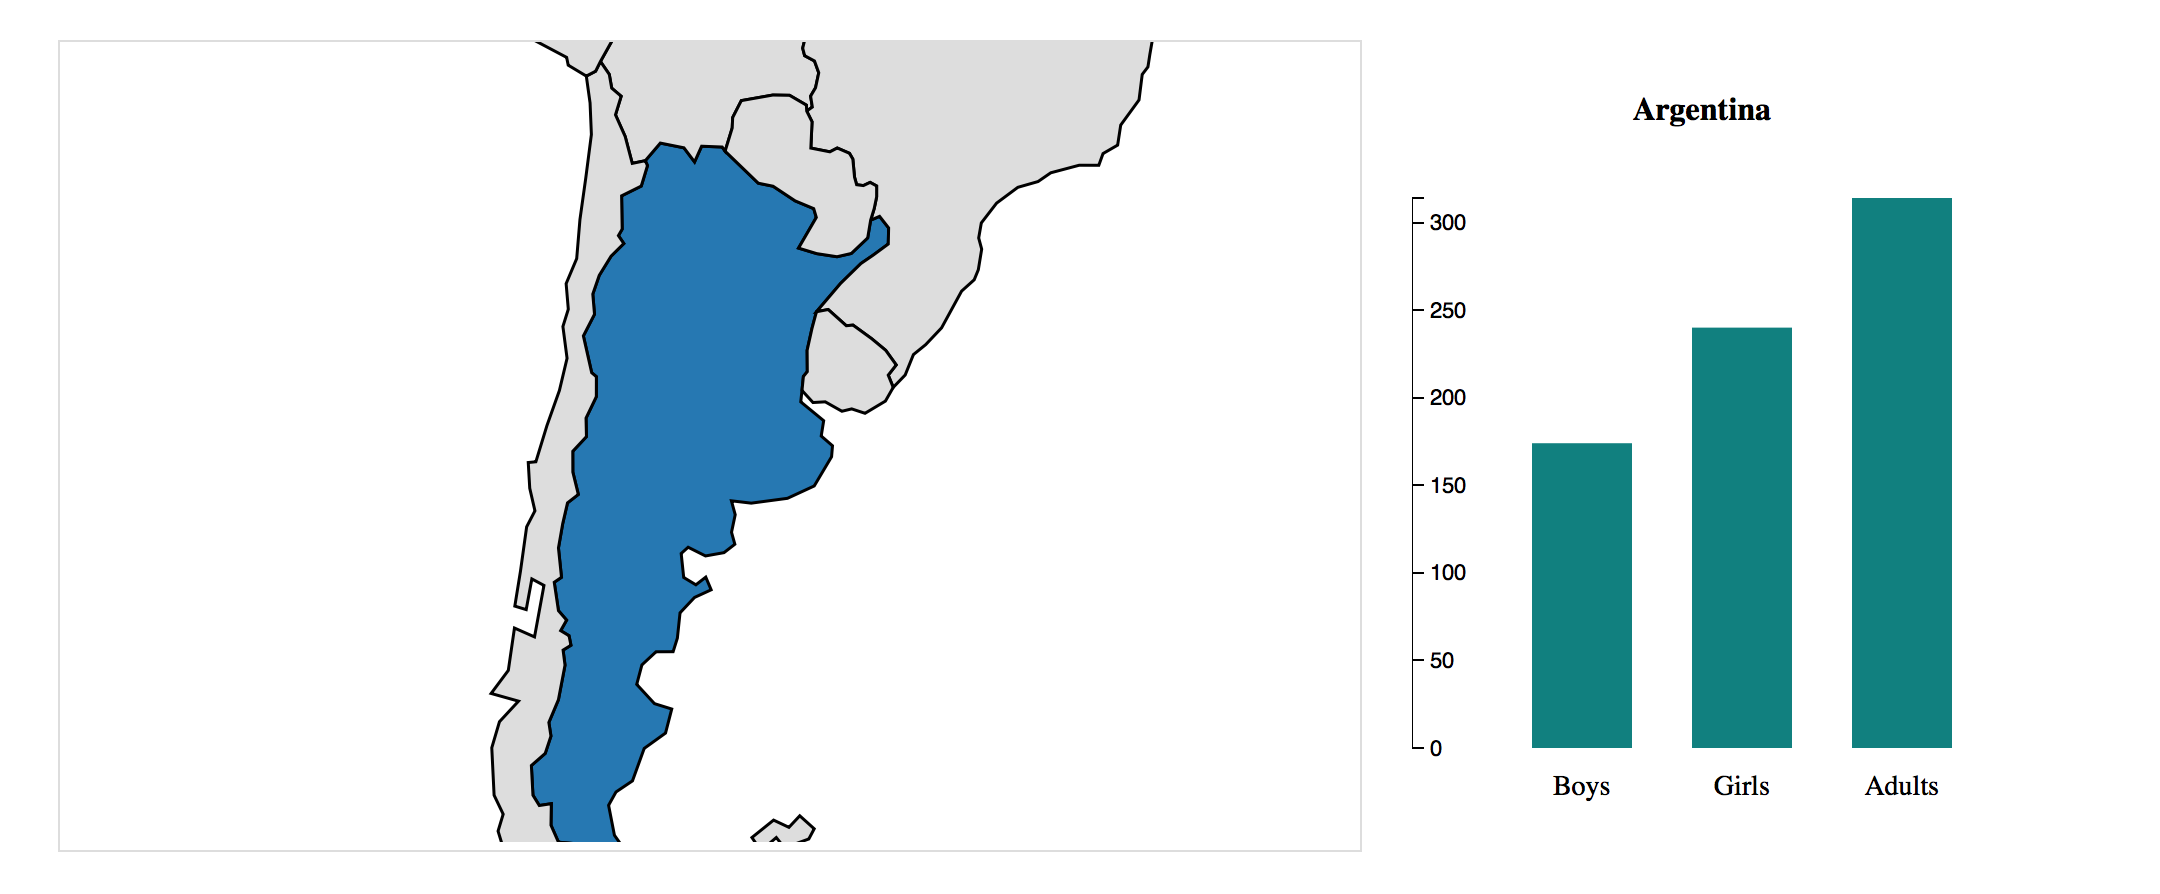
\includegraphics[width=0.7\textwidth]{5.png}
\caption{\label{fig:5} Country and its data in the barchart}
\end{figure}

\subsection{How we measure success}
We think that our success from a short-term perspective equals how much the community partner is satisfied. With this respect, we got a good feedback from the community partner: "This is wonderful to see. I love the map and the bar chart at the side!." This was a much better result than we expected. Still, the real success should not be measured only by the feedback: if our visualization increases real donors, then we can say our visualization is successful in a real sense.
\subsection{Experiment we conducted}
The performance of the visualization is probably one of the most important concerns since it totally can change the user experience and impression on the viusalization. Nobody will like visualizations that take more than, say, 30 seconds to show. We recognized that ours was not such a case, yet were interested in the actual performance. For this experiment section, we conducted to time the performance of our visualization, using the latest Chrome and Chrome Developer Tool (See, Figure 3 and 4). For every execution, internet cache was cleared. The measurement was carried out five times each on OS-X Yosemite and Windows 7. The results are visualized in Figure 5.

\begin{figure}
\centering
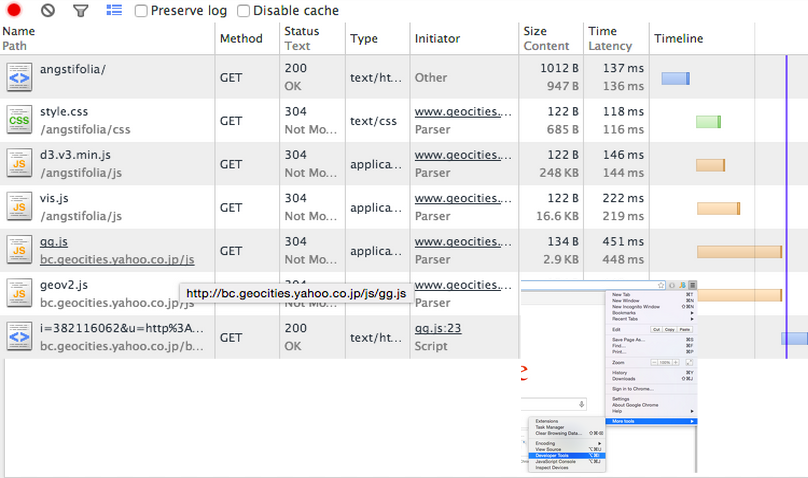
\includegraphics[width=0.4\textwidth]{1.png}
\caption{\label{fig:1}Chrome Developer Tool}
\end{figure}

\begin{figure}
\centering
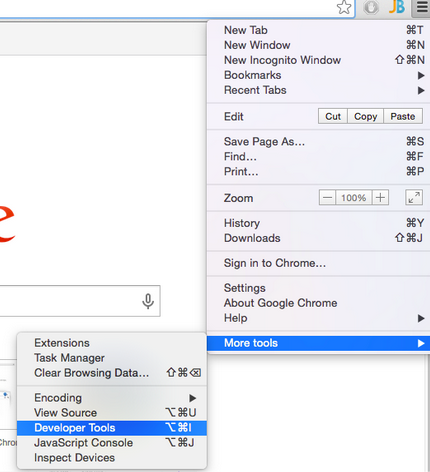
\includegraphics[width=0.4\textwidth]{2.png}
\caption{\label{fig:2}How to run the tool}
\end{figure}


\subsection{What our results indicate}
Regardless of the OS, the execution speed is all less than 0.4ms. Since our implementation relies on vis.js to add and manipulate DOM elements and show visualizations, these results mean that ours are fast enough. That is, they do not harm the user experience. Perhaps, the size of the data contributed to this good performance: small data does not take much time to be processed. 
\begin{figure}
\centering
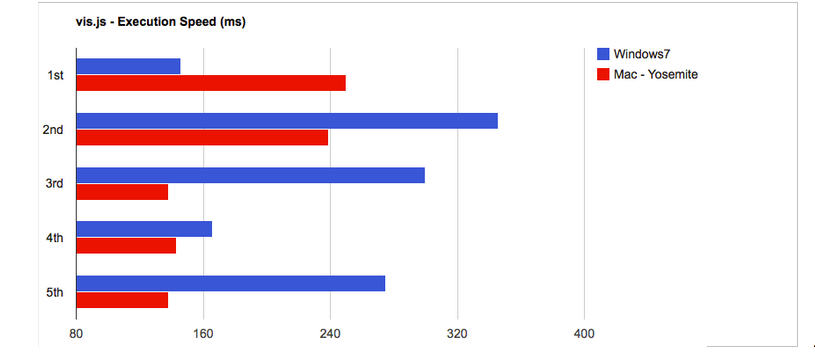
\includegraphics[width=1.0\textwidth]{3.png}
\caption{\label{fig:3}Experimental Result}
\end{figure}



\section{Discussion}
\subsection{Is our approach promising?}
We hope so, but it is not clear unless real users evaluate our visualization and give feedbacks to us.

\subsection{Possible different or better approaches}
One possible approach is to use a bigger map, and merge charts totally into it. This is what we discussed in an early section. If this approach is possible, the design consistency of the visualization can increase, and we may be able to get a better responce from the user, comparing to just putting the map to the left side and charts to the right side. Another possible approach is to use multiples charts. This is a straightforward way. Although this approach has a weakness that the user does not necessairly check each chart, it is still easy to implement and maintain.

\subsection{What we learned from this project}
First, we should not assume that our community partner has the same knowledge with us: the partner is not necessarily familiar with the computer and programming. It will probably be the best to avoid using of technical terms (e.g., debugging) when to ask the partner about the project or report the progress. Second, it is import to consider how our product will be used. In class assignments, we basically do not need to care about some aspects of programs such as maintenance, deployment or future updates. Yet, in this project, the situation is totally different. Considering those aspects is essential to be successful.

\subsection{What we would do if we could start the project again}
If we could start the project again, we would show some samples such as design sketches on paper to the community partner first. Fornatunately, this time, we could get a good feedback from the partner without showing such a sample, yet if we had shown, we may be able to delineate what the partner really wanted. 

\section{Conclusion}
We have worked with our community partner, One World in this project so far. We experienced a lot of trial and errors, yet finaly could go through creating a visualization, which we hope to achieve the goal of our partner. During this project, we realized that communication with the client can be more important than coding. As mentioned in an early section, we needed to recreate our visualization from scratch because once we failed to find out the exact needs of the partner. We both did and learned a lot, but miscommunication still can happen. it can not only lose our time but also make the project difficult to be successful. Fortunately, this project seems to end without more troubles. We hope we can apply what we learned to future projects and visualization projects.


\end{document}